%
% The first command in your LaTeX source must be the \documentclass command.
\documentclass[sigchi]{acmart}

\usepackage[]{algorithm2e}
\usepackage{tabularx}
\usepackage{geometry}
\usepackage[utf8]{inputenc}

\geometry{margin=1in}


%
% defining the \BibTeX command - from Oren Patashnik's original BibTeX documentation.
\def\BibTeX{{\rm B\kern-.05em{\sc i\kern-.025em b}\kern-.08emT\kern-.1667em\lower.7ex\hbox{E}\kern-.125emX}}
    
% Rights management information. 
% This information is sent to you when you complete the rights form.
% These commands have SAMPLE values in them; it is your responsibility as an author to replace
% the commands and values with those provided to you when you complete the rights form.
%
% These commands are for a PROCEEDINGS abstract or paper.

%
% These commands are for a JOURNAL article.
%\setcopyright{acmcopyright}
%\acmJournal{TOG}
%\acmYear{2018}\acmVolume{37}\acmNumber{4}\acmArticle{111}\acmMonth{8}
%\acmDOI{10.1145/1122445.1122456}

%
% Submission ID. 
% Use this when submitting an article to a sponsored event. You'll receive a unique submission ID from the organizers
% of the event, and this ID should be used as the parameter to this command.
%\acmSubmissionID{123-A56-BU3}

%
% The majority of ACM publications use numbered citations and references. If you are preparing content for an event
% sponsored by ACM SIGGRAPH, you must use the "author year" style of citations and references. Uncommenting
% the next command will enable that style.
%\citestyle{acmauthoryear}

%
% end of the preamble, start of the body of the document source.
\begin{document}

%
% The "title" command has an optional parameter, allowing the author to define a "short title" to be used in page headers.
\title{High-level abstraction of image editing features}

%
% The "author" command and its associated commands are used to define the authors and their affiliations.
% Of note is the shared affiliation of the first two authors, and the "authornote" and "authornotemark" commands
% used to denote shared contribution to the research.
\author{Brandon Cuadrado}
\email{brandon.cuadrado@stonybrook.edu}
\affiliation{%
  \institution{Stony Brook University}
  \streetaddress{TBD}
  \city{Stony Brook}
  \state{New York}
  \postcode{11790}
}

%
% By default, the full list of authors will be used in the page headers. Often, this list is too long, and will overlap
% other information printed in the page headers. This command allows the author to define a more concise list
% of authors' names for this purpose.
\renewcommand{\shortauthors}{B. Cuadrado}

%
% The abstract is a short summary of the work to be presented in the article.
\begin{abstract}
High-level image processing is a task of artistic merit which requires a high-level of expertise in the field. Manipulating 2D images using color transfer, image enhancement, and other techniques have applications in both photorealistic and non-photorealistic areas of image manipulation. This report will cover the synopsis and evaluation of the implementation of this technique to create a functional image processing architecture for a breadth of high-level techniques and features. This model can automatically extract the color palette of an input image, which the user can then alter and produce an output image via a user-selected color palette. This parsed image can also be edited via image enhancement and color harmonization, which may then be applied to aesthetically-adjacent groups of images with the databasing of image features within a robust object-oriented design.
\end{abstract}

%
% The code below is generated by the tool at http://dl.acm.org/ccs.cfm.
% Please copy and paste the code instead of the example below.
%

%
% Keywords. The author(s) should pick words that accurately describe the work being
% presented. Separate the keywords with commas.


%
% A "teaser" image appears between the author and affiliation information and the body 
% of the document, and typically spans the page. 
\begin{teaserfigure}
  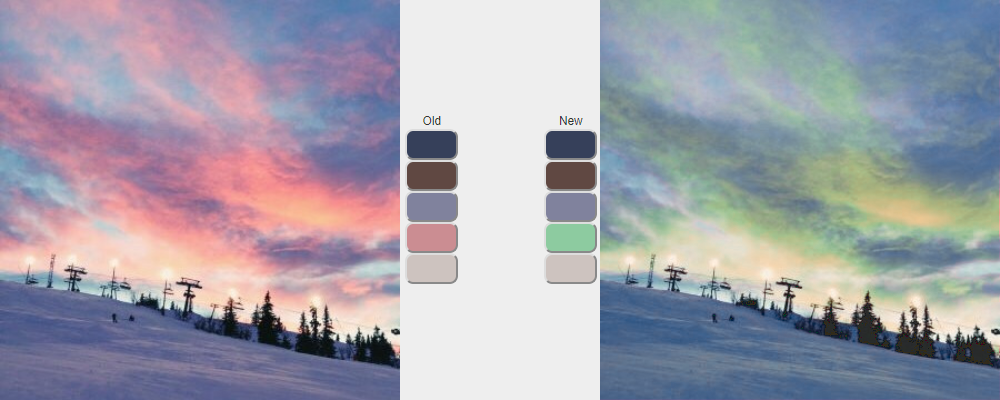
\includegraphics[width=\textwidth]{SkyTeaser.png}
  \caption{Palette-based color transformation}
  \Description{Placeholder.}
  \label{fig:teaser}
\end{teaserfigure}

%
% This command processes the author and affiliation and title information and builds
% the first part of the formatted document.
\maketitle

\section{Introduction}
Image processing techniques that manipulate images at a semantic level traditionally require expertise in the field. In the age of social media, the demand for accessible image processing techniques rises. In an effort to relieve the existing difficulty of image processing, algorithms at the semantic and data-driven level can provide an automated approach to image processing. High-level image processing techniques can be made accessible to colloquial users through the combination of efficient image processing algorithms and intuitive interface design.

In an early iteration of this dashboard, the model achieves color transfer via the extraction of a representative palette of colors for the image. Colors within a palette can be edited to a new color, thus mapping all associated colors to the appropriate transferred value. This concept of palette-based image processing is extended to a comprehensive feature set, consisting of color, pixel location, luminance mapping, and other image features. These features can be manipulated by the user in a manner derivative from palette-based color mapping to perform high-level transformations via a simplified dashboard.

Expanding the palette-based abstraction of feature mapping to other high-level image processing processes enhances the existing methods of automating these tasks in a number of ways.

\begin{itemize}
	\item{\textbf{Feature-set abstraction}}: Allow high-level concepts to be abstracted into intuitively manageable features.
	\item{\textbf{Interface}}: Provide machine-agnostic web-based interface for performing high-level image processing techniques.
	\item{\textbf{Extensible architecture}}: Feature-based architecture allows for abstraction of other image editing data into similarly compartmentalized structures.
\end{itemize}

\section{Related Work}
\noindent\textbf{Palette-based Photo Recoloring.} The work of Chang et. al. inspired the algorithms for Palette-based Color Transfer. The concept of extracting a palette from an input image introduces the feature abstraction concept that permeates the entire project. The method of color palette extraction used in this work employs a modified version of the K-Means Clustering algorithm. Once a palette is extracted from the input image, the colors are converted to LAB color space and color transfer is performed on the a and b values, with luminance calculated in an independent transform. 
\linebreak

\noindent\textbf{Color Harmonization.} Color Harmonization, as described in the work of Cohen-Or et. al., is the process of transferring colors in an image to produce an output that contains aesthetically pleasing color combinations. The harmonic templates used to describe suitable color combinations are represented in ranges across a circular hue wheel. Determining a harmonic scheme that corresponds with a given input image involves measuring the harmony of an image with respect to each harmonic scheme. The user may also determine a manual choice of the output harmonic scheme. This research also defines a function used to recolor images, similar to the task described in Palette-based photo recoloring.
\linebreak

\noindent\textbf{Image recoloring using geodesic distance-based color harmonization.} This work from Li et. al. extends upon previous existing Color Harmonization frameworks by adding geodesic distance calculations onto state-of-the-art color harmonization methods of the time. Geodesic distance is applied to reassign hues outside of the harmonic scheme, once the most harmonious scheme has been selected. This method of assigning colors to new values allows most colors within the image to remain unchanged. Thus, color harmonization can be applied with minimal interference to image semantics.
\linebreak

\noindent\textbf{Group-Theme Recoloring for Multi-Image Color Consistency.} The work by Nguyen et. al. proposes a method of editing the colors within multiple images to share the same aesthetic. The framework achieves color consistency for multiple images by establishing a group color theme for input. Using a palette-based approach, this architecture establishes extracted palettes from the input images. To achieve color consistency among a group of images, a group color theme is computer and each image palette is modified accordingly.
\linebreak

\noindent\textbf{Histogram Equalization: A Strong Technique for Image Enhancement.} This work by Singh and Dixit describes methods of image enhancement using modified Histogram Equalization techniques. This is achieved by partitioning images into segments and performing equalization functions separately in the image. This applies more semantic significance to the traditional histogram equalization algorithm. The methods of Dynamic Histogram Equalization and Contrast Limited Adaptive Histogram Equalization are discussed, along with their usefulness and drawbacks.

\section{Methodology}

\subsection{Palette Extraction}

Automatically extracting the palette from an image is achieved using a modified version of the K-Means Clustering algorithm. The goal is to select k colors that are representative of the colors in the original image. The choice of  is selected by the user, with options ranging between 3 and 6 colors.

This algorithm takes the pixels in an input image and assigns each to a bin. The bins are organized in a 3-dimensional histogram of size 16 x 16 x 16. Each dimension of the histogram represents a color channel in RGB space. Once each color has been assigned a bin, the mean color is computed in Lab color space. The mean colors collected here are the points used for calculating the K-Means centroids.

\begin{figure}[t]
	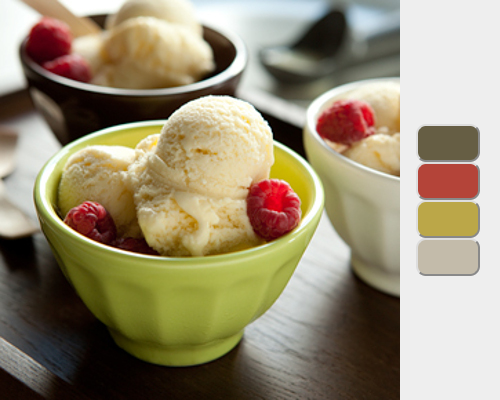
\includegraphics[width=8cm]{IceFigure}
	\caption{4-k image palette extraction}
\end{figure}

To initialize centers, the k-largest bins are determined and their means are used as initial centers. This results in uniform palette output through each attempt at extracting a palette, as opposed to using random centers to start. In order to put less emphasis on near-black colors, an additional black centroid is included in the k-means algorithm. As such, a k-sized palette uses k+1 centroids. Once K-Means Custering is applied to these values, the output centers are used as the extracted image palette.

\subsection{Color Transfer}

Transferring colors between palettes requires a combination of luminance mapping and hue transfer. This calculation is performed in Lab color space. The method used in this iteration preserves the luminance value between input and output pixels. As such, only the a and b values of color mapping are changed.

To change colors from the original palette to the output palette, the algorithm operates on a and b values in Lab color space. Lab color space gamut represents the domain of valid color values given the range of the three L, a, and b values. As such, a transform is performed between the a and b values within the constraints of a constant L value. In the case that the resulting color is outside of the valid Lab color gamut, an additional function is performed to fit the color transform within the gamut.

This process is repeated for all color changes between the input and output palettes. These changes are they applied to a pixel by weighing the transform for each color in the palette. This algorithm treats each individual color in the image as a weighted combination of the colors in the associated palette. Once applied to every pixel, the color transform process is complete.

\subsection{Histogram Equalization}

Histogram Equalization in the style of Dynamic Histogram Equalization uses image features to define the behavior of classic image editing techniques. In the case of Dynamic Histogram Equalization, after determining the histogram of the entire image, local minima are extracted. These are used to divide the image and assign gray levels to each partition. Traditional histogram equalization is then applied to each partition individually.

The intensity of the resulting equalized image can be adjusted within the dashboard by applying a weight to the amount of contrast. Additionally, the number of partitions may also be customized for results that fit most semantically with the image contents.


\subsection{Color Harmonization}

The proposed algorithm from Cohen-Or et al. considers each pixel of an image in finding the best appropriate harmonic scheme. To abstract this architecture to conform to a simplified feature set, we can apply harmonic fitting to an extracted palette. Thus, an image's color palette, which represents the image as a whole, can provide a simplified and streamlined view of the image when finding the best harmonic scheme.

In the updated model, a palette color's hue, saturation, and the template's sector border among the harmonic scheme are considered when calculating the image's harmony value, with respect to a given template. This matches the algorithm followed in the original proposal, but abstracted to be applied only to the image's parsed palette.



\section{Technical Details}

\subsection{Web-based Razor MVC}

The Image Processing Dashboard is developed with Microsoft Visual C\# using Razor MVC to develop a front end with JavasSript and JQuery. All image processing tasks are performed on the server side with a custom built object-oriented architecture representing and manipulating image features.

Using HTML and CSS, the interface allows for a custom user image to be uploaded to the system. Processing the image for its features initiates server-side code to store and parse image pixel, color, and luminance data within the image processing architecture. 


\begin{figure}[t]
	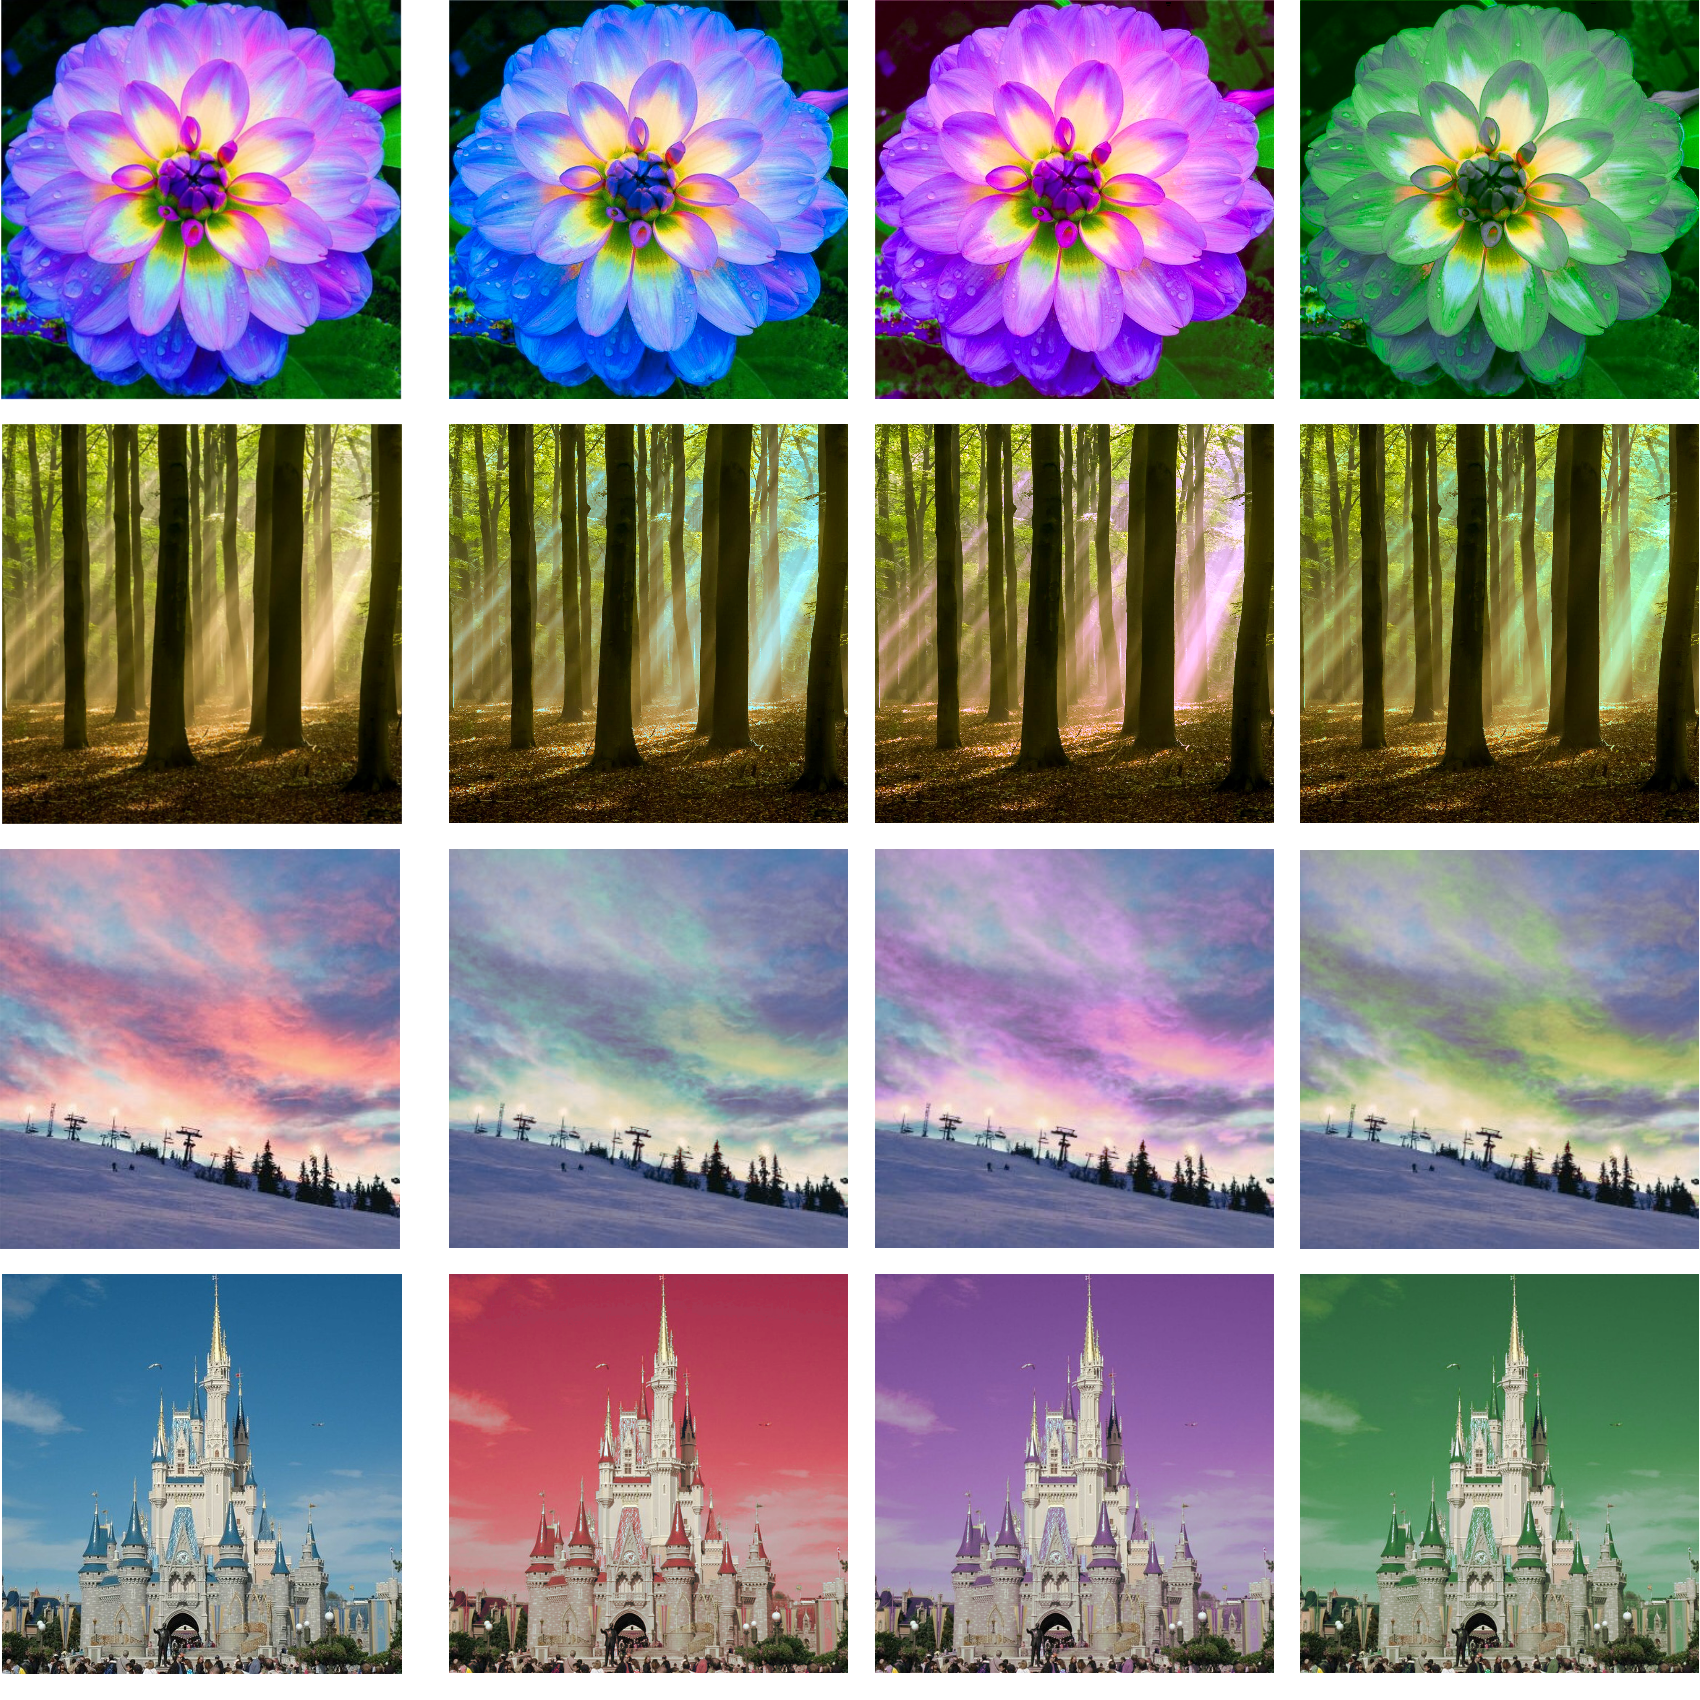
\includegraphics[width=8cm]{Diffs}
	\caption{Color transfer output using Palette-based iteration.}
\end{figure}

\subsection{Palette-based Iteration}

The initial iteration of the dashboard solely implemented Palette-based Color Transfer, based on the research of Chang et. al. This early version of the dashboard set the standard of architecture to hold future features to come. Custom Image, Palette, Color, Pixel, and other image processing feature object classes were created in C\# to support the various general components of image processing tasks. This would allow further tasks to be performed on a shared C\# object-oriented architecture.

Following the Color Transfer algorithm detailed in Section 3, a transfer function is applied to each palette color that has been changed. Assume the original palette color is \(C\), the new palette color selected by the user is \(C'\) and the function representing the difference between these colors is \(f_1\). Let us also say that the pixel to perform palette-based color transfer on is \(x\) and the desired output pixel is \(x'\). The simplest calculation would be to apply the distance between \(C'\) and \(C\) to all pixels of value \(x\). This, however, can cause the color to result outside of the Lab color space gamut; thus causing invalid values. Snapping these values to the closest in-gamut value would result in rough transitions between colors in the image. As such, two cases of color transfer need to be considered.

The simple "far" case is applied when the function \(x_0-x+C'-C\) is in gamut. If so, \(x_b\) is calculated as the point where a parallel ray intersects with the gamut boundary. In the "near" case, the \(x_0\) value results in an out of gamut color. Thus, \(x_b\) is instead calculated as the boundary intersect from a ray from \(C'\) to \(x_0\). With these values, the resulting \(x'\) is calculated using the following formulation:

\[\frac{||x'-x||}{||C'-C||}={\Big(1,\frac{||x_b-x||}{||C_b-C||}\Big)}\]

In both cases, the resulting \(x'\) will be within the Lab color gamut. With this function, colors that lay outside of the Lab color gamut will smoothly transition between values that blends into the semantics of the scene. To apply this function \(f(x)\) to a list of palette colors, we treat the function of \(f_i(x)\) where \(i\) represents the index of a palette color. Using a weight coefficient, the each function output can be combined to output the resulting pixel. The transfer function looks as follows:

\[f(x)=\sum_{i}^{k}w_i(x)f_i(x) \mid \sum_{i}^{k}w_i(x)=1\]

The weights are calculated using radial basis functions representing weights for each color in the palette. The radial basis function is performed using a Gaussian kernel. As described in Chang et al.'s study, this kernel results in a smooth and accurate representation of the colors' make-up. As a means of accelerating image computation, the radial basis functions are always calculated at the time of palette generation.


\begin{algorithm}
	\caption{Color Transfer}
	\KwData{new\_palette;}
	\KwResult{Recolored image;}
	\ForEach{color c in new\_palette}{
		Use RBF to find weight function \(w_c(x)\);
	}
	
	\ForEach{pixel p in image}{
		Perform \(f(p)\);
	}
\end{algorithm}

\subsection{Extended Feature-Set}

By taking the design principles of a palette-based color transfer model, high-level image processing tasks can be abstracted to manageable pieces for the average user. This architecture principle can be applied to many of the processing tasks discussed in this project to be included in a comprehensive dashboard.

\subsection{Image Enhancement}

Image enhancement via Histogram Equalization is a technique that is easily abstracted to fit this model. The traditional implementation of this technique already requires little interaction from the user, besides the potential to indicate a threshold of impact that the process outputs. As such, the concept of histogram equalization inherently fits into this architecture's core value.

To perform traditional histogram equalization in this architecture, a list of luminance values of every image pixel is parsed in Lab color space. This list is then normalized between 0 and 100 across the spectrum of luminance values. Consider a list \(L\) representing all luminance values in an image, where \(l_{max}\) represents the maximum value across all luminance values in the image. In Lab color space, the ratio between the original and current values can be calculated with the following equation:

\[r=\frac{100}{l_{max}}\]

With the ratio \(r\), each luminance value, \(l_i\) can be multiplied by \(r\) to find its new value, \(l'_i\).

\[l'_i=r \times l_i\]

\begin{figure}[t]
	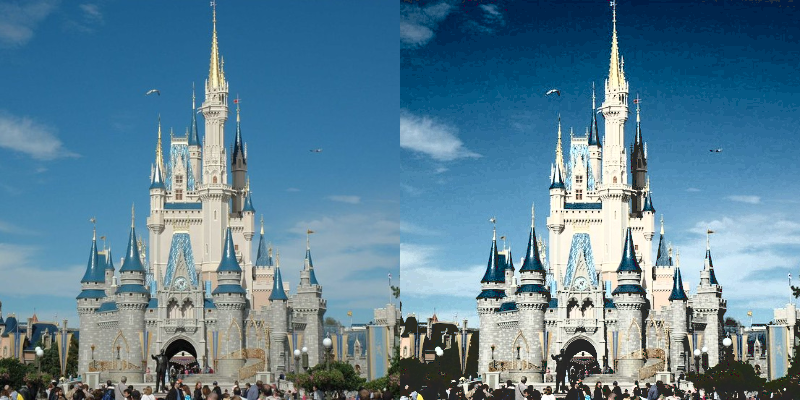
\includegraphics[width=8cm]{CastleCompare}
	\caption{Histogram Equalization applied to an image}
\end{figure}

\subsection{Color Harmonization}

Regarding Color Harmonization, the existing Color Harmonization algorithm of Cohen-Or et al. can be refactored to make use of the Palette-based color transfer architecture. Namely, extracted palettes can be matched with a harmonic scheme in a similar fashion to the original model. Using an extracted palette, we can use the function \(F(X, (m,\alpha))\) to find the harmony of an image \(X\) with the harmonic scheme represented by \((m,\alpha)\), where \(m\) represents the harmonic template and \(\alpha\) represents the associated orientation. Rather than iterate through all pixels in the image, we can perform this operation for each color in the image's palette.

\[F(X,(m,\alpha)) = \sum_{c \in X} \Big|\Big| H(c) - E_{T_m(\alpha)}(c) \cdot S(c) \Big|\Big|\]

In the above operation, \(H\) and \(S\) denote the hue and saturation channels, respectfully. The \(||\cdot||\) operation represents the arc-length distance on the hue wheel in radians. \(E_{T_m(a)}(c)\) represents the sector border hue of template \(T_m\) with orientation \(\alpha\) closest to the hue of palette color \(c\).

Once there is a measure for harmony using solely palette colors, the remaining steps of the algorithm can be performed as originally proposed. Namely, finding the best harmonic scheme of the image \(X\) under the template \(T_m\), such that the value of the angle \(\alpha\) minimizes \(F(X,(m,\alpha))\).

\[M(X,T_m)=(m,\alpha_0) \text{   s.t.   } \alpha_0= argmin_{\alpha}\Big(F\big(X, M(X,\alpha)\big)\Big)\]

Following this step, the best harmonic scheme \(B(X)\) of the image \(X\) is determined by minimizing the \(F\) function over all templates \(T_m\).

\[B(X)=(m_0,\alpha_0) \text{   s.t.   } m_0= argmin_{m}\Big(F\big(X, M(X,T_m)\big)\Big)\]

\section{Evaluation}

In this paper, performance is evaluated with respect to various aspects. Firstly, the project has made improvements from traditional Palette-based Color Transfer methods given its changes to luminance mapping. This aspect of improvements can be evaluated via quality of output and efficiency of the algorithm. Additionally, we can evaluate the interface updates and expansions to usability. this user experience lens can be expanded to evaluate the interaction between other image editing tasks added to the dashboard. Lastly, as alluded to in the user experience evaluation points, the project's custom architecture, with respect to palette-based features, additional feature abstraction, and feature extensibility, can be evaluated.

With respect to the refactorizations made in our palette-based color transfor algorithm, there are three main aspects to the changes presented in this paper:

\begin{itemize}
	\item{\textbf{Luminance mapping}}: the change in Luminance in Lab color space has been refactored in an attempt to present semantically-consistent color transitions within an image.
	\item{\textbf{Tech stack}}: The Microsoft Visual Web Development stack is used to enhance communication between front and back-end in an intuitive way. This increases efficiency from the previous client-side iteration.
	\item{\textbf{Extensible architecture}}: The architecture introduced in the latest iteration provides extensibility toward other feature, in addition to robust manipulation within the scope of palette-based transformations.
\end{itemize}

Luminance mapping impacted palette-based color transfer by both reducing the time to execute the algorithm and reducing the difference between input and output pixel colors. This attempts to better represent the semantics of an image between results, while keeping true to the luminance of the original image. 

Updates to the tech stack, pertaining to the migration from a purely JavaScript framework to server-side C\# image arithmetic, resulted in an approximately 50\% faster time for color transfer computation. The updated stack allows for user experience improvements as well, as computation no longer freezes the web interface for the duration of the color transfer algorithm.

The custom architecture built in Microsoft Visual C\# provides improvements to both the algorithm and scope of the project. By adopting an object-oriented architecture, the runtime of image editing algorithms becomes noticeably decreased from that of a client-side algorithm using solely scripting. This improvement provides a more robust and reliably manipulation of image features, as well. Features can be editing at a higher level than previous iterations, with information no longer constrained to the limitations of a canvas element in HTML.

\section{Future Work}

The scope of this project lies in its ability to expand upon existing image-editing tasks, allowing for usable and robust manipulations of high-level feature. The current iteration of the project provides an extensible framework for representing high-level features in an object-oriented architecture. While the current iteration sets this baseline, future work would be required to make expansions to the scope of this framework.

This object oriented architecture paves the way for databasing edited images at the feature-level, rather than the pixel-level. This high-level representation of images can be expanded upon to create a database of features between images, all represented in this modular, object-oriented design. This current iteration is designed to act as a single node that, with time, can be a single element within a network of high-level, semantic image editing features.


\section{Conclusion}

The abstraction of image editing features to fit within an object-oriented design paves the way for databasing and manipulating high-level image editing tasks through robust, automated methods. The work in this project sets the groundwork for representing images through features, rather than pixel values, in a method designed to keep semantics relevant at the raw data-driven level of design. With further extension of this groundwork, in addition to fleshed out image-editing tasks formatted to this architecture, this project can provide a means of editing images in a robust, feature-driven framework. Additionally allowing for databasing in a robust way, while maintaining the same consideration to semantics as demonstrated in the codebase itself.

\nocite{*}
\bibliography{Bibliography}
\bibliographystyle{acm}



\end{document}
